\chapter{研究背景}
\label{chap:haikei}

本章では楽譜の問題点と、楽譜を扱う既存システムの現状を整理する。

\newpage

\section{楽譜}

楽譜は楽曲を記号や文字によって書き表したものである。
一般に五線譜のことを指すことが多いが、ギター演奏用に利用されるタブ譜や日本固有の三味線譜など、用途やジャンル、地域によって様々な種類の楽譜が存在する。
西洋音楽をルーツに持つ五線譜は国際的かつ普遍的なものとして認められており、現在は様々な音楽を記録するために広く利用されている。

\section{楽譜の歴史}

本節では今日利用されている楽譜が生まれるまでの進化の歴史を概観する\cite{Minagawa}。

\subsection{ネウマ譜}
ネウマ譜(図\ref{neume})は旋律の上行下行の動きをネウマと呼ばれる線状の記号で表示する記譜法で、9世紀頃から中世キリスト教会の典礼音楽であったグレゴリオ聖歌の記譜のために用いられはじめた。
10-11世紀ごろからは横線(譜線)を添えて、音程関係を明確にする試みが行われた。
譜線が添えられている限りは音高が明確だが、リズムの表示はあいまいである。

\begin{figure}[H]
    \centering
    \includegraphics[width=7cm]{images/neume.png}
    \caption{ネウマ譜の例}
    \label{neume}
\end{figure}

\subsection{定量譜}
複数の奏者がそれぞれ異なった声部を同時に演奏する多声音楽が生まれると、リズム表示があいまいな従来のネウマ譜では不十分となった。
13世紀後半になると、音の長短を音符の形状で区別する定量譜(図\ref{teiryo})が利用されるようになった。

\begin{figure}[H]
    \centering
    \includegraphics[width=9cm]{images/teiryo.png}
    \caption{定量譜の例}
    \label{teiryo}
\end{figure}

\subsection{奏法譜}
15世紀ごろからは特定の楽器の演奏法を具体的に表示する奏法譜(図\ref{tab})も広く利用された。
楽器ごとに固有の奏法譜をもち、現代でも「タブ譜」としてギター演奏に利用されている。

\begin{figure}[H]
    \centering
    \includegraphics[width=6cm]{images/tab.png}
    \caption{奏法譜の例}
    \label{tab}
\end{figure}

\subsection{近代譜}
17世紀初頭から現在までに世界で最も普及している楽譜の形態(図\ref{kindai})で、鍵盤楽器用の奏法譜をルーツに持つ。
\begin{itemize}
    \item 五線による音高表示
    \item 音符の「はた」によるリズム表示
    \item 小節線の使用
\end{itemize}といった特徴がある。

\begin{figure}[H]
    \centering
    \includegraphics[width=9cm]{images/kindai.png}
    \caption{近代譜の例}
    \label{kindai}
\end{figure}

\subsection{現代音楽}
五線譜は鍵盤楽器をベースにした西洋音楽に最適化された記譜法のため、半音以下の繊細な音程のゆれや微妙なニュアンスを表現できないという制約がある。
現代の作曲家たちはそれぞれ独自の方法で克服しようと試みている(図\ref{kondo})。

\begin{figure}[H]
    \centering
    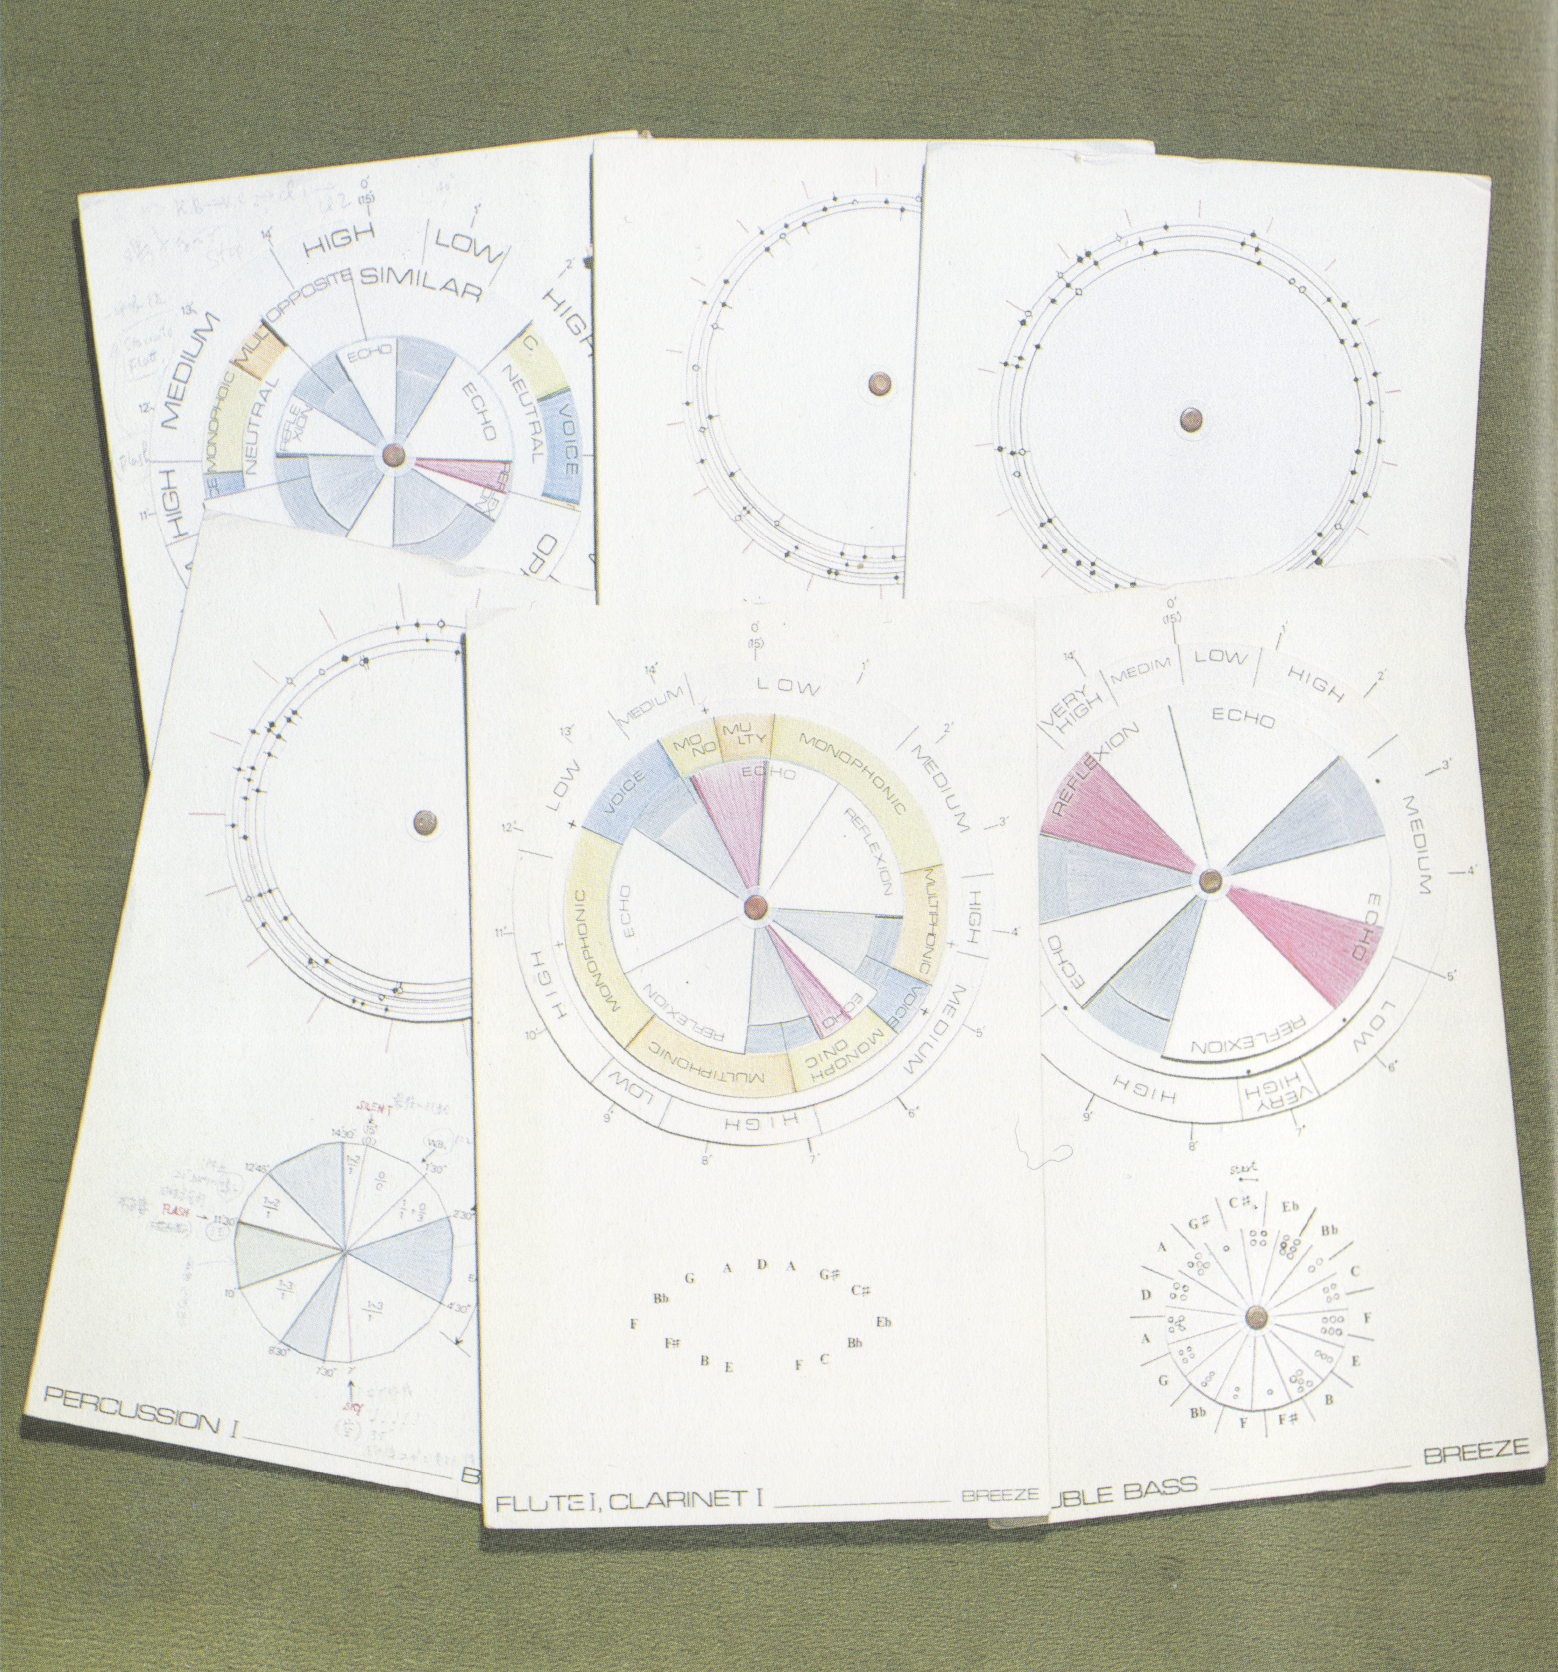
\includegraphics[width=9cm]{images/kondo.png}
    \caption{現代音楽譜の例}
    \label{kondo}
\end{figure}

\section{テキストの進化}
楽譜同様に紙の上で利用されていたテキストの進化にも注目する。
計算機が普及する以前のテキストは印刷物であるという制約から以下のような問題が存在した。
\begin{itemize}
    \item 簡単に編集できない
    \item せいぜい挿絵や写真程度の情報しか一緒に記録できない
    \item ドキュメントが複数存在するとき参照や管理が面倒
\end{itemize}

しかし現在では計算機の進化によりこれらの問題は完全に解決されている。
\begin{itemize}
    \item 手軽な編集\\
    計算機上でテキストを扱えるようになり、コピー/ペースト/Undo/Redoといったテキスト編集支援機能を搭載した各種エディタによって手軽な編集が可能になった。
    また印刷レイアウトを簡単に構成できるワープロソフトによって、美しいレイアウトの文章を簡単に作れるようになった。
    \item 手軽な入力\\
    日本語入力などの文字変換をサポートするシステム(IME)などによって手軽な入力が可能になった。
    \item マルチメディアの活用\\
    画像/音声/動画といったマルチメディアを自在に埋め込むことができるハイパーテキスト(図\ref{hy})によって、情報量の多いドキュメントの作成が可能になった。
    \item ハイパーリンク\\
    ハイパーテキストでは文章間リンクを示すハイパーリンク機能が利用でき、関連情報への素早いアクセスが可能になった。
    \item Web\\
    インターネット技術の進化とWebの普及によって、世界中に存在する様々なドキュメントへ瞬時にアクセスすることが可能になった。
    \item 共同編集\\
    Wikiのようなコラボレーションツールによって、場所や人数に制約を受けない共同編集が可能になった。
\end{itemize}


\begin{figure}[H]
    \centering
    \fbox{\includegraphics[width=9cm]{images/wikipedia.png}}
    \caption{ハイパーテキストの例}
    \label{hy}
\end{figure}

\section{楽譜の問題点}
\label{mondai}
一方、楽譜の性質は計算機の普及後も印刷物の時代から進化しておらず、以下のような問題が存在する。
\begin{enumerate}
    \item 簡単に編集できない\\
    現在流通している楽譜は紙やPDF形式での配布が一般的であり、内容の変更は前提とされていない。
    また自分で楽譜を書く場合は楽譜作成ソフトを利用できるが、印刷を前提としたレイアウトでの編集を強制されるため、一部だけアレンジしたい・1フレーズだけメモしたいといった用途には向いていない。
    \item メモなどの情報を自在に書けない\\
    楽譜を利用する際には、
    \begin{itemize}
        \item 演奏時に気付いたこと
        \item 演奏時に気をつけるべきこと
        \item 先生に習ったこと
    \end{itemize}などのメモを書き込みながら使うのが一般的である(図\ref{memo})。
    メモ書きできるのは余白スペースだけであり、楽譜自体に編集を加えてレイアウトを変更したり、音声や動画といった文字以外の情報を埋め込むことも不可能なので、記述できる内容は必然的に限られる。
    \item 参照や管理が面倒\\
    紙やPDFはそれぞれが独立しているため、手元の楽譜が増えると管理に苦労する。
    ファイル名でしか楽譜の内容を判断できないため、作曲者別にフォルダを分割するといったファイルの階層的な整理が必要である。
    また楽器構成や年代といった別の側面から参照したい場合には別途索引を用意しなければならない。
\end{enumerate}

\begin{figure}[H]
    \centering
    \fbox{\includegraphics[width=10cm]{images/fuga.png}}
    \caption{楽譜上のメモの例}
    \label{memo}
\end{figure}

\section{既存の楽譜システム}
現在広く利用されている楽譜利用システムを解説する。
\subsection{楽譜作成ソフト}
Finale\footnote{\textsf{https://www.finalemusic.jp/}}(図\ref{finale})、Sibelius\footnote{\textsf{http://www.sibelius.jp/}}といった楽譜作成ソフトがデファクトスタンダードとして商用・私用問わず広く利用されている。
スタンプ感覚で音符を入力できるWYSIWYGな編集環境を持ち、以下のような楽譜作成支援機能を利用できる。
\begin{itemize}
    \item 楽譜スキャン・OCR
    \item パート譜自動作成
    \item レイアウトの細かい微調整
\end{itemize}

\begin{figure}[H]
    \centering
    \includegraphics[width=10cm]{images/finale.png}
    \caption{Finaleの画面}
    \label{finale}
\end{figure}

\subsection{楽譜ビューアー}
ほとんどの楽譜はPDFファイルとして配布されるため、閲覧のために標準のPDFビューアーが利用されることが多い。
またPiascore\footnote{\textsf{http://piascore.com/}}(図\ref{pia})を代表とするタブレット端末向けの楽譜に特化したビューアーも広く普及しており、
\begin{itemize}
    \item 楽譜への書き込み
    \item 自動譜めくり
    \item メトロノーム
\end{itemize}といった機能を利用できる。

\begin{figure}[H]
    \centering
    \fbox{\includegraphics[width=8cm]{images/piascore.png}}
    \caption{Piascoreの画面}
    \label{pia}
\end{figure}

\section{まとめ}
楽譜の編集や閲覧を支援するシステムが広く利用されているが、これらは計算機上で楽譜の利用形態を再現したに過ぎず、
\begin{enumerate}
    \item 簡単に編集できない
    \item メモなどの情報を自在に書けない
    \item 参照や管理が面倒
\end{enumerate}という本質的な楽譜の問題は解決されていない。
次章では上記のような楽譜が持つ問題点を解決し、これまでの楽譜の在り方にとらわれない次世代の楽譜システム「ハイパー楽譜システム」を提案する。
